\documentclass[tikz, preview]{standalone}

\usepackage{amsfonts, amsthm, amssymb, amsmath, stmaryrd, etoolbox}
\usepackage{tikz}
\usetikzlibrary{matrix,arrows}

\begin{document}
\[
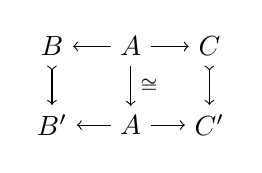
\begin{tikzpicture}
\node (B) at (-1,1) {$B$};
\node (A) at (0,1) {$A$};
\node (C) at (1,1) {$C$};
\node (B') at (-1,0) {$B'$};
\node (A') at (0,0) {$A$};
\node (C') at (1,0) {$C'$};
%
\draw [->] (A) edge (B);
\draw [font=\scriptsize,->] (A) edge node[right] {$\cong$} (A');
\draw [->] (A) edge (C);
\draw [->] (A') edge (B');
\draw [->] (A') edge (C');
\draw [>->] (B) edge (B');
\draw [>->] (C) edge (C');
\end{tikzpicture}
\]
\end{document}
